%Template generated by Ben Manning
%Purdue University
%btmannin@purdue.edu
%Last modified: 7/7/2021


\documentclass[notitlepage, 12pt]{report}  %The document class will setup a lot of basic formatting.  Report class will start with justifying paragraphs setup your different types of sections.

%Different packages allow you to add more functions that will make your time in LaTeX easier.
\usepackage{amsmath}
\usepackage{graphicx}
\usepackage{caption}
\usepackage{url}
\usepackage{circuitikz} % circuit drawer

%\usepackage{biblatex} %Imports biblatex package
\usepackage[style=numeric]{biblatex}
\addbibresource{bib.bib}

\usepackage[top=2cm, bottom=2cm, left=2cm, right=2cm]{geometry}

\title{Experiment 3 Report}

\begin{document}
%Everything needs to begin and end.  
\graphicspath{{./images/}}

\begin{center}
\large \textbf{Experiment 3 Report} \\ %\large and \small can help make text sizes vary throughout your document.
%\textbf will bold the text that is in the curly brackets
\small 
Andrew Lykken\\
Anna Kishnani\\
2 February 2023\\
Section 004 (Abraham Yakisan)\\
%\rule{500pt}{.1pt} 

\end{center}

% space between title and abstract
\vspace{4in}


\begin{abstract}
abstract here 
\end{abstract}

\newpage

\section*{Task 1} %Each task has a section including (but not limited to) Objective, 
% Procedure, Results / Calculations, Conclusions


\subsection*{Objective}

\indent\indent The objective of this task is to measure $V_{t}$ by using an operational amplifier to self-adjust 
the gate-source voltage such that it is exactly $V_{t}$. \\

\subsection*{Procedure}

\indent\indent This circuit is built around the ALD1106 quad PMOS transistor chip. This chip is very prone to being
damaged through electrostatic discharge. Because of this, when working with this chip, a grounded antistatic 
wristband was worn.\\

\textbf{Step 3-4}

The circuit below was built

\begin{center}
    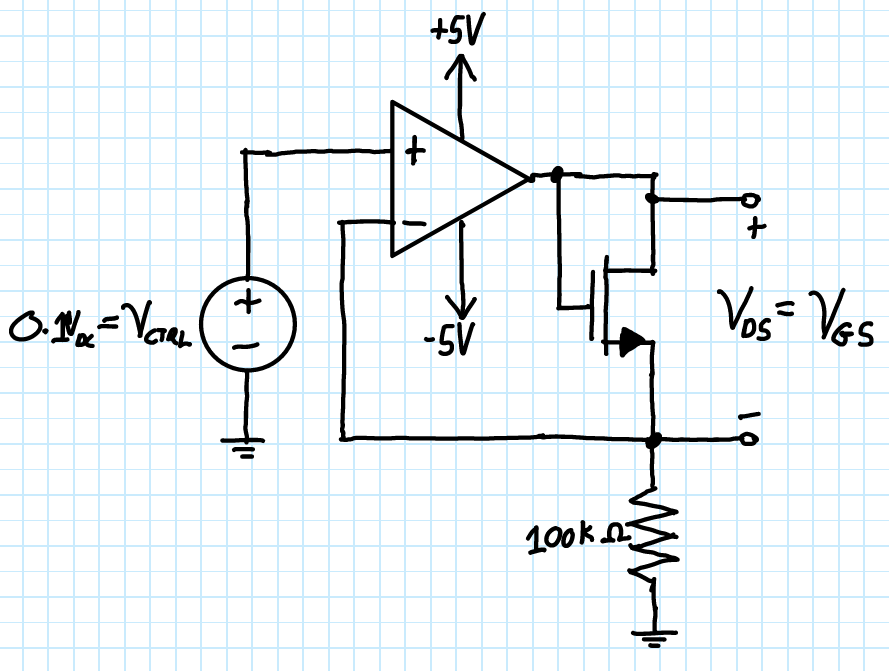
\includegraphics[scale=0.35]{fig3.2.png}
\end{center}

using a control voltage of 0.1V as to set a constant current through the transistor of 1$\mu$A.\\

\textbf{Step 5}

The voltage across the 100k$\Omega$ resistor was measured to ensure the value of the drain current was what 
was expected. \\  

\textbf{Step 6-7}

The voltage $v_{GS}$ was measured to be the threshold voltage of the transistor, then the circuit was built around 
the other 3 transistors present in the ALD1106 chip, and the threshold voltages were measured and recorded.\\

\textbf{Step 8-9}

These threshold voltages were then compared against the threshold voltages listed on the ALD1106 datasheet.



\subsection*{Results / Calculations}

\textbf{Step 5}
When measuring the voltage across $R_s$, the 100k$\Omega$ resistor, the value measured was 99.3 mV. \\

Using:\\
\begin{equation}
    V = IR 
\end{equation}
\begin{equation}
    v_{Rs} = i_D * R_s
\end{equation}
we can find the current $i_D$ by rearranging and filling in known values:\\

\begin{equation}
    i_D = \frac{v_{Rs}}{R_s} = \frac{99.3 mV}{100k\Omega} = 0.993\mu A
\end{equation}

which is very close to the desired current value $i_D = 1\mu A$. \\

\textbf{Step 6-8}

The threshold voltages $V_t$ were measured for each transistor in the ALD1106 chip.
The position description relies on the chip being placed with the divet on the top. Each of the 
transistors correspond to a corner of the chip when placed in this configuration, which is how
they are described in the table below. \\

\begin{table}[h!]
    \begin{center}
        \begin{tabular}{c|c}
            Transistor Position & $V_t$ $(v_{GS})$ \\
            \hline
            Top Left            & 0.607V           \\
            Bottom Left         & 0.611V           \\
            Top Right           & 0.600V           \\
            Bottom Right        & 0.608V          
        \end{tabular}
    \end{center}
\end{table}

The transistors have very similar threshold voltages, differing by a maximum of 0.011V, or 1.8\% of the average value.

\textbf{Step 9}

The datasheet for the ALD1106 chip states that the threshold voltage shall not be greater than 1V, not 
lower than 0.4V, and is typically 0.7V.\cite{datasheet} \\

These transistors' threshold voltages hover around 0.6V, which is slightly lower than typical, but definitely
within a reasonable margin of the specifications.\\

\subsection*{Conclusions}

\indent\indent In \textbf{Task 1}, an ALD1106 chip was tested to determine each of its component transistors' threshold voltages. 
The circuit was designed to have a very low drain current, which was effective in our physical circuit, measuring 
very close to the design specification. Each threshold voltage for the transistors were very similar to each other, 
and were within tolerance for the chip's design. \\

\section*{Task 2}

\subsection*{Objective}


\indent\indent The objective of this task is to create multiple $i_d$ - $v_{DS}$ curves at various $v_{GS}$ values, to calculate 
the transconductance parameter $k_n$ for a transistor in the ALD1106 chip.\\


\subsection*{Procedure}

\textbf{Step 1-3}

The circuit below was built and connected to the Analog Discovery 2 using the ports described:

\begin{center}
    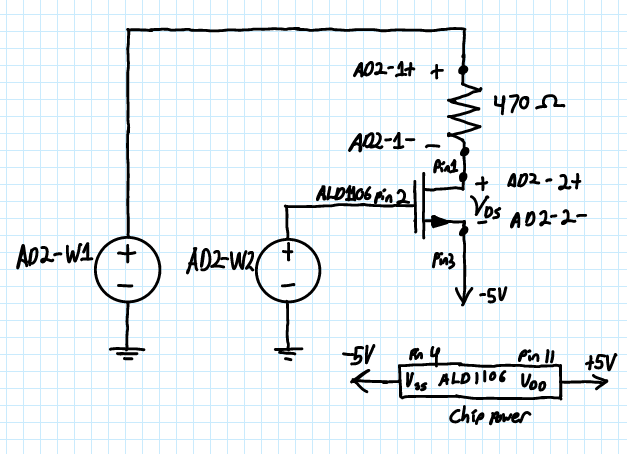
\includegraphics[scale=0.5]{task2_circuit.png}
\end{center}

\textbf{Step 4-10}

The Analog Discovery 2 has a tracer function to compute I-V characteristic curves for various components. \\

The Tracer tool was opened in WaveForms. The following parameters were set:

\begin{itemize}
    \item The device was set to ``N-FET''.
    \item ``No Adapter'' was selected in the adapter menu.
    \item In the ``Options'' dropdown, ``Emitter'' was set to -5V.
    \item The ``Measure'' parameter was set to ``Id/Vds''. 
    \item The Curve Tracer was configured to measure $v_{GS}$ from 0V to 5V in 500mV steps.
    \item The Curve Tracer was configured to sweep $v_{RD}$ from 0V to 10V. 
    \item ``$R_d$'' was set to 470$\Omega$. 
\end{itemize}


The tracer was then run to produce a graphical representation of the I-V characteristic of this transistor. \\

\textbf{Step 11}

The graph produced from \textbf{Step 10} was used to calculate the transconductance parameter, $k_n$. 

\subsection*{Results / Calculations}

\textbf{Step 1-9} 
The circuit was implemented on a breadboard and measured through WaveForms. \\

\textbf{Step 10}

The following is the graph generated from WaveForms' tracer tool with the parameters defined in \textbf{Procedure}. \\

\begin{center}
    \includegraphics[scale=0.5]{Task2_graph.png}
\end{center}

\textbf{Step 11}

Using the graph above, the transconductance parameter $k_n$ can be calculated using:

\begin{equation}
    i_{D(sat)} = \frac{k_n}{2} * (v_{GS} - V_t)^2
\end{equation}

where a point on any curve is taken in the saturation region. \\

Using the point on the curve where $v_{GS}$ = 5V, $i_D$ = 5.5 mA, and $v_{DS}$ = $v_{GS}$ - $V_t$ = 4.293V, the value for $k_n$ can be calculated. 
Note that $v_{DS}$ does not actually matter for the calculation, however it is important in knowing that this point 
lies in the saturation region of operation. The threshold voltage $V_t$ is used from \textbf{Task 1: step 6}. \\

With these values known, the equation becomes:

\begin{equation}
    k_n = \frac{2 i_D}{(v_{GS} - V_t)^2} = \frac{2 * 0.0055 A}{(5V - 0.607V)^2} = 0.57 \frac{mA}{V^2}
\end{equation}

This is repeated for each $v_{GS}$ curve, using the current $i_D$ at the $v_{DS}$ value equal to $v_{GS} - v_t$. The results follow:

\begin{table}[h!]
    \begin{center}
        \begin{tabular}{c|c|c}
            $v_{GS}$ (V) & $i_D$ (mA)& $k_n$ ($\frac{mA}{V^2}$) \\
            \hline
            0V           & 0 mA   & DNE    \\
            0.5V         & 0 mA   & DNE    \\
            1V           & 0.1 mA & 1.2    \\
            1.5V         & 0.3 mA & 0.75   \\
            2V           & 0.7 mA & 0.721  \\
            2.5V         & 1.3 mA & 0.7255 \\
            3V           & 1.9 mA & 0.663  \\
            3.5V         & 2.7 mA & 0.645  \\
            4V           & 3.5 mA & 0.608  \\
            4.5V         & 4.5 mA & 0.593  \\
            5V           & 5.5 mA & 0.569 
        \end{tabular}
    \end{center}
\end{table}

\subsection*{Conclusions}
In this task, $k_n$ was estimated by testing the transistor at various $v_{GS}$ values, and recording the current and drain-source voltage. 
This method worked very well, producing consistent and accurate results. Estimating for very low $v_{GS}$ values was difficult due to the
scale of the data generated, but as the voltage became more reasonable, the results became more and more clear. \\

\newpage

\printbibliography[title={\Large References}] %Prints out the bibliography sources that you have used in the document.

\end{document}